\chapter{Cross-lingual Word Sense Disambiguation}
\label{sec:clwsd}

Cross-lingual word sense disambiguation (CL-WSD) is the task of labeling words
or phrases in some input text with their contextually-appropriate translations
into some target language.
It is a variant of the more general WSD task, with the sense inventory for each
word defined as its possible translations.
This setting for WSD has immediate applications in both machine translation and
cross-language information retrieval, since many words have multiple possible
translations.

WSD in translation has a long history; practical work in integrating
WSD with statistical machine translation dates back to early SMT work at IBM
\cite{Brown91word-sensedisambiguation}, but the problem itself was described in
Warren Weaver's prescient 1949 memorandum \cite{weavermemo}, which describes an
essentially modern conception of word sense disambiguation.

In the early history of machine translation, researchers were very concerned
with WSD; to some, it seemed an insurmountable problem. Bar-Hillel 
discussed the difficulty of writing a program to translate sentences with
simple ambiguities like \emph{The box was in the pen.} \cite{barhillel1960}:

\begin{quote}
... I know of no program that would enable a machine to come up with this
unique rendering unless by a completely arbitrary and ad hoc procedure whose
futility would show itself ...
\end{quote}

To produce a correct rendering of this sentence in Spanish, for example, the
translation system must decide between translating ``pen" as \emph{corral} (an
enclosure, like for an animal) or as \emph{pluma} (the instrument for writing).
As of this writing, for this particular example, Google Translate picks the
less-sensible ``in the writing implement" translation (see Figure
\ref{fig:box-in-pen}).
One wonders how this could come about -- we would hope that the n-gram language
model for Spanish would prefer sentences about things in enclosures to things
in writing implements.
But the word \emph{en} can be a translation of either the English ``in" or
``on", and \emph{pluma} can also mean ``feather".
The situation is fairly complex.


\begin{figure}
  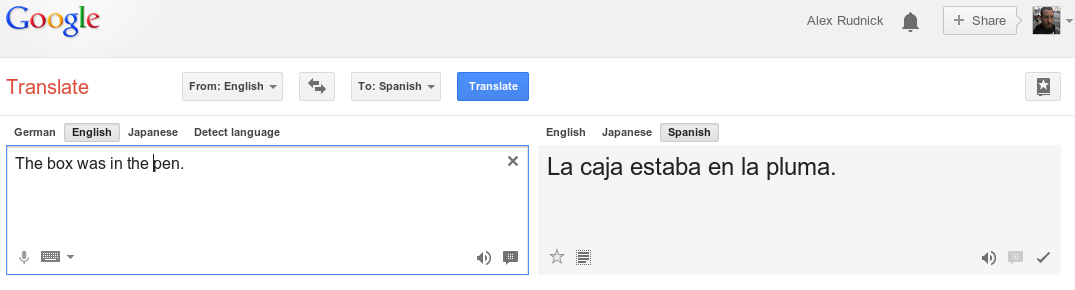
\includegraphics[width=12cm]{box-in-pen.png}
  \caption{Google Translate, September 17, 2013; interestingly, adding or
  removing the final period in the English sentence causes a switch between the
  ``pluma" and ``corral" renderings.}
  \label{fig:box-in-pen}
\end{figure}

In general, there is a many-to-many relationship between words across language
boundaries.
This happens for a number of reasons: figurative or metaphorical uses may not
translate directly,
obligatory information in one language may be left unspecified in another,
or the criteria for selecting a word may simply differ.
To give some familiar examples, a ``leg" of a trip in English is typically
translated as \emph{etape} in French, which is unrelated to limbs used for
walking;
translating ``brother" to Japanese requires specifying whether the brother is
older (\emph{ani}) or younger (\emph{ot\=oto});
a soap bubble or a ceramic plate can be destroyed with the same word in
Chinese, whereas English speakers typically distinguish between the verbs
``pop" and ``break" \cite{majid2007semantic}.

Despite these difficulties, most statistical MT systems do not use an explicit
WSD module \cite{wsdchap3}; the language model and phrase tables of these
systems mitigate lexical ambiguities by encouraging words used collocationally
to appear together in the output. Entire phrases\footnote{Not necessarily
``phrases" in a syntactic sense, but subsequences of sentences} such as verbs
with their common objects may be learned and stored in the phrase table, and
the language model will encourage common collocations as well.

To take a look at some apparently easier examples, let us also consider the
following usages of \emph{letter}, from the test set of a recent SemEval shared
task \cite{task10}, and how to translate them into Spanish.

\enumsentence{
But a quick look at today's \emph{letters} to the editor in the Times suggest
that here at least is one department of the paper that could use a little more
fact-checking. }
\label{sent:carta}
\enumsentence{
All over the ice were little Cohens, little Levys, their names sewed in block
\emph{letters} on the backs of their jerseys. }
\label{sent:letra}

We would want (\ref{sent:carta}) to be translated with the word \emph{carta},
and (\ref{sent:letra}) to be translated with \emph{letra} or something similar.
Google Translate (as of this writing) handles both of these sentences well,
rendering the first with ``cartas" and the second with an even better choice,
translating the phrase ``block letters" as \emph{mayúsculas}.
However longer-distance relationships, search errors, or simple statistical
accidents can still cause strange translations in practice.

Despite the great success of SMT systems without any explicit models for WSD,
there has been recent interest in CL-WSD and its application to translation
systems, sparking shared tasks at recent SemEval workshops
\cite{lefever-hoste:2010:SemEval,task10} and a number of other projects
described in some detail in \S\ref{sec:relatedwork}).

In this dissertation, we will describe in detail some new approaches for CL-WSD
and how to integrate them into a practical machine translation system.
We will develop and extend at least two broad approaches for CL-WSD: the use of
multilingual evidence where available, and CL-WSD as a sequence labeling
problem.
Both of these techniques have been prototyped and presented at workshops, but
they will be refined significantly and packaged into more general tools for use
in MT.  

\begin{figure}
  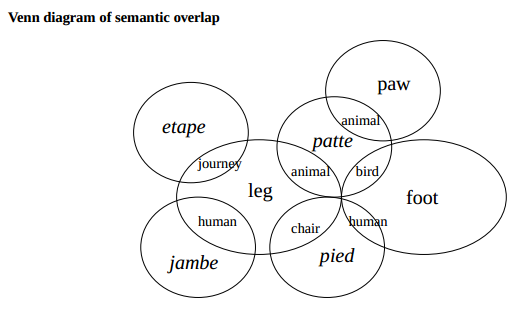
\includegraphics[width=12cm]{hutchins-leg-etc.png}
  \caption{Overlap of words related to ``leg"; relationships between English
  and French words. Figure 21.2 from \protect\cite{slp1}; example originally
  from \protect\cite[Chapter 6]{hutchins1992introduction}.}
  \label{fig:leg}
\end{figure}

\section{Using multilingual evidence}
For some languages, such as English, Spanish, and the other languages of the
European Union, we have multiple bitext corpora available, covering several
different language pairs with the same source language. Through the Europarl
corpus \cite{europarl}, for example, we have bitext corpora in which English is
paired with Spanish, German, French, and 17 other European languages.
We would like to be able to make use of evidence from all of these corpora when
translating into any particular target language, ideally even when the corpora
involved are not all mutually parallel.
Each corpus may contain useful examples of a given source language word,
and senses of that word may be lexicalized in varying, non-overlapping ways in
the different target languages.
This approach is particularly informed by the ongoing work of Els Lefever
\emph{et. al} (see especially \cite{lefever-hoste-decock:2011:ACL-HLT2011}),
although their technique requires an entire machine translation system to
perform CL-WSD, which seems unwieldy when we want to use CL-WSD as a
subcomponent of a machine translation system.

We want a CL-WSD system to be able to learn the relationships between the
senses of a given source word that are lexicalized in different ways in various
languages.
Two target languages may happen to surface the same sense distinctions, perhaps
due to being related languages, or simply by coincidence.
Alternatively, a combination of translations into several languages may provide
evidence for a certain lexical choice in the target language of interest.

In early 2013, we developed a prototype CL-WSD system that makes use of
multilingual evidence \cite{rudnick-liu-gasser:2013:SemEval-2013} and produced
some of the best results in a SemEval shared task on CL-WSD \cite{task10}.
Concretely, teams undertaking the task had to translate polysemous nouns from
English into five other European languages.
In our SemEval paper, we presented three variations on the approach:
a straightforward classification approach (without multilingual evidence), a
classifier stacking approach, and a graphical model system based on loopy
belief propagation over Markov networks.

The simplest system presented in that work, based on a maximum entropy
classifier, simply extracted features from a window around the English noun to
be translated and used these to make a prediction. The same system could also
return a probability distribution over target language words or phrases. This
simple system was used as a subcomponent in the two more sophisticated systems.

\subsection{Classifier stacking}
The classifier stacking approach, in order to predict the translation of a word
into a given target language, uses translations into the other four available
target languages as features.
For example, to translate an English word into Spanish, we would give the
classifier features encoding that word's translations into French, Italian,
Dutch and German.
At training time, since we were provided with parallel translations for all six
languages, we found the correct answers in the parallel corpora, but for test
sentences, the translations were not available, so they were predicted with the
simpler non-multilingual classifiers.

The classifier stacking approach could likely be improved by adding features
derived from more sources.
We would like to try adding classifiers trained on the other Europarl
languages, as well as completely different corpora; this would require that for
the stacked classifier, we would train on predicted translations rather than
This approach only requires that the first-layer classifiers make \emph{some}
prediction based on text in the source language;
they need not be trained from the same source text, depend on the same
features, or even output words as labels. Monolingual WSD systems seem likely
to help out, as do Brown-style word clusters \cite{brown1992class}.

\subsection{Markov Networks}
In our SemEval entry, we also investigated a Markov network (or ``Markov Random
Field") approach, building a network of interacting variables (see Figure
\ref{fig:pentagram}) to solve the classification problem for all five target
languages jointly.

The network has nodes that correspond to the distributions produced by the
simple classifiers, given an input sentence, and edges with pairwise potentials
that are derived from the joint probabilities of target language labels
occurring together in the training data. 
Thus the task of finding the optimal translations into five languages jointly
is framed as a MAP inference problem, where we try to maximize the joint
probability of all five variables, given the evidence of the features extracted
from the source language sentence.
The inference process is performed using loopy belief propagation
\cite{DBLP:conf/uai/MurphyWJ99}, which is an approximate but tractable
inference algorithm that, while giving no guarantees, often produces good
solutions in practice.
We used the formulation for pairwise Markov networks that passes messages
directly between the nodes rather than first constructing a cluster graph,
which is described in \cite[\S 11.3.5.1]{Koller+Friedman:09}.

\begin{figure}
  \begin{center}
  \includegraphics[width=5cm]{pentagram.pdf}
  \end{center}
  \caption{The network structure used in the MRF system: a complete graph with
  five nodes, in which each node represents the random variable for the
  translation into a target language.}
  \label{fig:pentagram}
\end{figure}

Our initial approach for setting the weights in the Markov network requires,
for each pair of languages, a parallel corpus for that language. It thus seems
less easily extensible than the classifier stacking approach, in which it is
clear how we can include all kinds of heterogeneous information.
The benefit of the Markov network approach is that it takes seriously the
uncertainty present in the predictions of each of the component classifiers,
solving the entire problem jointly.
The Markov network approach may also play a part in our future CL-WSD systems.

\subsection{CL-WSD as a Sequence Labeling Problem}
We will also investigate the use of sequence models for CL-WSD.
The intuition behind the sequence labeling approach is that machine translation
implies an ``all-words" WSD task, in that we need to choose a translation for
each word in the source sentence, and that the sequence of translations chosen
should make sense when taken together.

We have developed a prototype CL-WSD system based on sequence labeling and
applied it to both English-Spanish and Spanish-Guarani translation tasks.
Concretely in this case, we want to label each source language word with a
target language word or phrase, or \emph{NULL}.
This work was presented at the HyTra workshop in August
\cite{rudnick-gasser:2013:HyTra-2013}.

One promising formalism for this line of work, used in the prototype, is the
Maximum Entropy Markov Model \cite{icml00/mccallum}.
Like an HMM, an MEMM models transitions over labels, although in the MEMM the
input sequence is given.
This frees us to extract any features we like from the source language
sentence. The ``Markov" aspect of the MEMM is that, unlike a standard maximum
entropy classifier, we can include information from the previous $k$ labels as
features, for a $k$-th order MEMM.
Thus at every step in the sequence labeling, we want a distribution
$P(t_i | S, t_{i-1}...t_{i-k})$ describing the probability of each possible
target-language label for the current source language token.
Here the probability of a sequence of labels $T$ is the product of each of the
individual transition probabilities that compose that sequence.
These probabilities are estimated with a MaxEnt classifier trained with 
the MEGA Model optimization package
\footnote{\url{http://www.umiacs.umd.edu/~hal/megam/}}.
For inference with this model, we used a beam search rather than the Viterbi
algorithm, for convenience and speed while using a second-order Markov model.

To avoid building a single classifier that might return
thousands of different labels, we could in principle build a classifier for
each individual word in the source language vocabulary, each of which will
produce perhaps tens of possible target language labels. However, there will be
tens or hundreds of thousands of words in the source language vocabulary, and
most word-types will only occur very rarely, especially in a low-resource
scenario.
In any case, it may be prohibitively expensive to train and store many
thousands of classifiers.

We would like a way to focus our efforts on some words, but not all, and to
back off to a simpler model when a classifier is not available for a given
word. It turns out to be straightforward to do this --  we can use MaxEnt
classifiers when available, and then use the simpler HMM when they are not. The
details of how to do this are described in the paper.

In the implementation, we can specify criteria under which a source language
word will have its translations explicitly modeled with a maximum entropy
classifier. When training a system, one might choose, for example, the 100 most
common polysemous words, all words that are observed a certain number of times
in the training corpus, or words that are particularly of interest for some
other reason.

At training time, we find all of the instances of the words that we want to
model with classifiers, along with their contexts, so that we can extract
appropriate features for training the classifiers. Then we train classifiers
for those words, and store the classifiers in a database for retrieval at
inference time.

%%At each step in the sequence, we would like the distribution over possible
%%labels for the current source word, given the source sentence features and the
%%recent context. If we had already estimated the parameters for an HMM, we could
%%compute the joint probability of each possible target 
%%$P(s_i, t_i | t_{i-1}...t_{i-k})$ -- 
%%as is typical in HMMs, it is just the product of the ``transition" and
%%``emission" probabilities, which are straightforward to estimate. To turn this
%%into a conditional probability, we could divide by the prior of the current
%%source word.
%%In the context of minimizing negative log-probabilities during beam search,
%%this is not necessary, since the source word is fixed; we can simply use the
%%negative log of that joint probability as-is.

We have yet to explore what the best approaches are for choosing which, and how
many, words should be modeled with classifiers for best results, but this will
be an important question to address.

More sophisticated sequence models, such as Conditional Random Fields
\cite{lafferty2001conditional}, may be useful in this task as well. 
We ran into difficulties in initial experiments with the off-the-shelf
CRF tool Mallet \cite{McCallumMALLET} -- training proved intractable on
one machine due to the large label space (all target-language words and
phrases), but these problems may be surmountable with some ingenuity or
parallelism.

\subsection{System Combination and Other Future Directions}
There are a number of future directions that we would like to investigate, in
addition to the ones mentioned previously.
Notably, we will do significant feature engineering; so far, the features we
have used for our classifiers have been limited to the tokens in a small window
around the current source word and their part-of-speech tags.
For the Spanish-Guarani language pair, we will be able to make use of
the comparatively large set of resources for analyzing the input Spanish.
We could extract many different features, perhaps syntactic ones through a
source language parser, word-cluster features for each input word, WordNet
synset labels (when available), bag-of-words features for the entire sentence,
or even discourse or document-level features where appropriate.

We will also develop ways to integrate different CL-WSD algorithms with each
other and with their containing MT systems; one obvious approach would be to do
classifier stacking from within an MEMM.
We could also imagine having an MT system invoking several different CL-WSD
systems and using them in an ensemble-like way.
Perhaps the CL-WSD systems could vote, with each of their recommendations
weighted using MERT, and leaving the final choice to the decoder.

We will also need to address both multi-word expressions and morphology and how
they interact with the CL-WSD system.
Thus far, we have assumed one-to-many alignments, and labeled each source word
with zero or more lemmatized target words or word stems.
However in practice, we will want to make use of multi-word expressions, and
our translation systems will need to generate appropriately inflected target
language text. This latter problem, and possible approaches for addressing it,
will be discussed in subsequent sections.

%The question we were trying to address is like:
%what if your n-gram model over labels for your source language has one idea
%(this is the next likely label), and your emission probabilities say something
%else (this is the label most likely to generate the observed input word)...
%well, we could imagine just making several different decisions and letting the
%decoder sort it out. We're doing that already actually, by including
%phrase-table probabilities and a language model.
%Are we just converging on the idea of a log-linear model again?
%But the point here is that we don't have to have just one CL-WSD system. We can
%have a bunch and let them fight it out. Hopefully this will help!
